\section{Trigonometric functions}

In this chapter, we'll learn about trigonometric functions, so functions whose argument is an angle. Examples for trigonometric functions are Sine, Cosine and Tangent. As we'll see later, these functions let us describe oscillations mathematically, and they are essential for any mathematical description of periodic functions --- which all musical notes are.

\begin{comment}

\subsubsection{Mathematical Description: Trigonometric Functions}

Trigonometric functions describe the relationship between angles and ratios of sides in triangles (originally right-angled triangles). They are fundamental for describing oscillations. One of the reasons why this is the case is because they are periodic, just like the oscillations we want to describe with them.

\paragraph{Definition of the Sine and Cosine Function}

The most important trigonometric functions are sine and cosine. They are special ratios of the side lengths in a right-angled triangle.
In a right triangle, the sine of an angle $\alpha$ is defined as:
\begin{align}
    \sin(\alpha) = \frac{\text{opposite }}{\text{hypotenuse}} \\  
    \cos(\alpha) = \frac{\text{adjacent}}{\text{hypotenuse}}
\end{align}

\paragraph{Radians and degrees}

\paragraph{Visualizing sine and cosine}
To get an idea what the Sine function actually looks like, we plot $\sin(x)$ as a function of the angle $x$ in radians.

As you can see in Fig. \ref{img:sinusfunktion}, the Sine function repeats after a period of $2\pi$. It is precisely this periodicity that makes it useful for describing oscillations.

\end{comment}

\subsection{Degrees and Radians}

Before we can begin our investigation of trigonometric functions, we need to talk about angles, as they are the argument of trigonometric functions.

There are two units in which you can state the value of an angle, degrees and radians. From school, you're probably already familiar with degrees, where a right angle corresponds to $90$ degrees, and a full circle corresponds to $360$ degrees. In this course, we'll use a radians, because this makes notation a bit easier. In radians, a right angle corresponds to $\pi/2$, and a full circle to $2\pi$. Thirty degrees are the same thing as $\pi/6$ radians, sixty degrees are the same as $\pi/3$ radians, etc. So:

\begin{itemize}
    \item \textbf{Degrees}: A full circle consists of $360^\circ$
    \item \textbf{Radians}: A full circle corresponds to $2\pi$
\end{itemize}

The conversion between both units is given by:
\begin{equation}
    360^\circ = 2\pi \quad \Rightarrow \quad 1^\circ = \frac{\pi}{180}
\end{equation}

The reason we choose $2\pi$ to be the value for the full circle is because the diameter of a circle is $2\pi$ times its  radius. So if you have a circle (let's say a circular cake) with radius one, and you cut out a piece with an angle of $\alpha$, the value of $\alpha$ will be exactly the length of the piece of crust on your piece. Neat, right?

This means that you can either describe an angle by its number of degrees or just by a number in radians. Angles are measured counterclockwise. 
Radians are especially important in higher mathematics because they simplify many formulas.

\subsection{Unit Circle}
A handy tool to visualize different angles and trigonometric functions is the unit circle. The unit circle is a circle with radius 1 centered at the origin. 
By Pythagoras' theorem, all points on the unit circle must satisfy 

\begin{equation}\label{eq:circ}
    x^2 + y^2 = 1
\end{equation}

You can test this by plugging in this equation into the graphing calculator of your choice, for example GeoGebra.
A drawing of the unit circle with some angles in degrees and in radians is given in Fig. \ref{fig:unit_circle}. For some points, their coordinates are also given.

\textit{Exercise: Check that the points of the coordinates in Fig \ref{fig:unit_circle} satisfy eq. \ref{eq:circ}.}

\begin{figure}
    \centering
    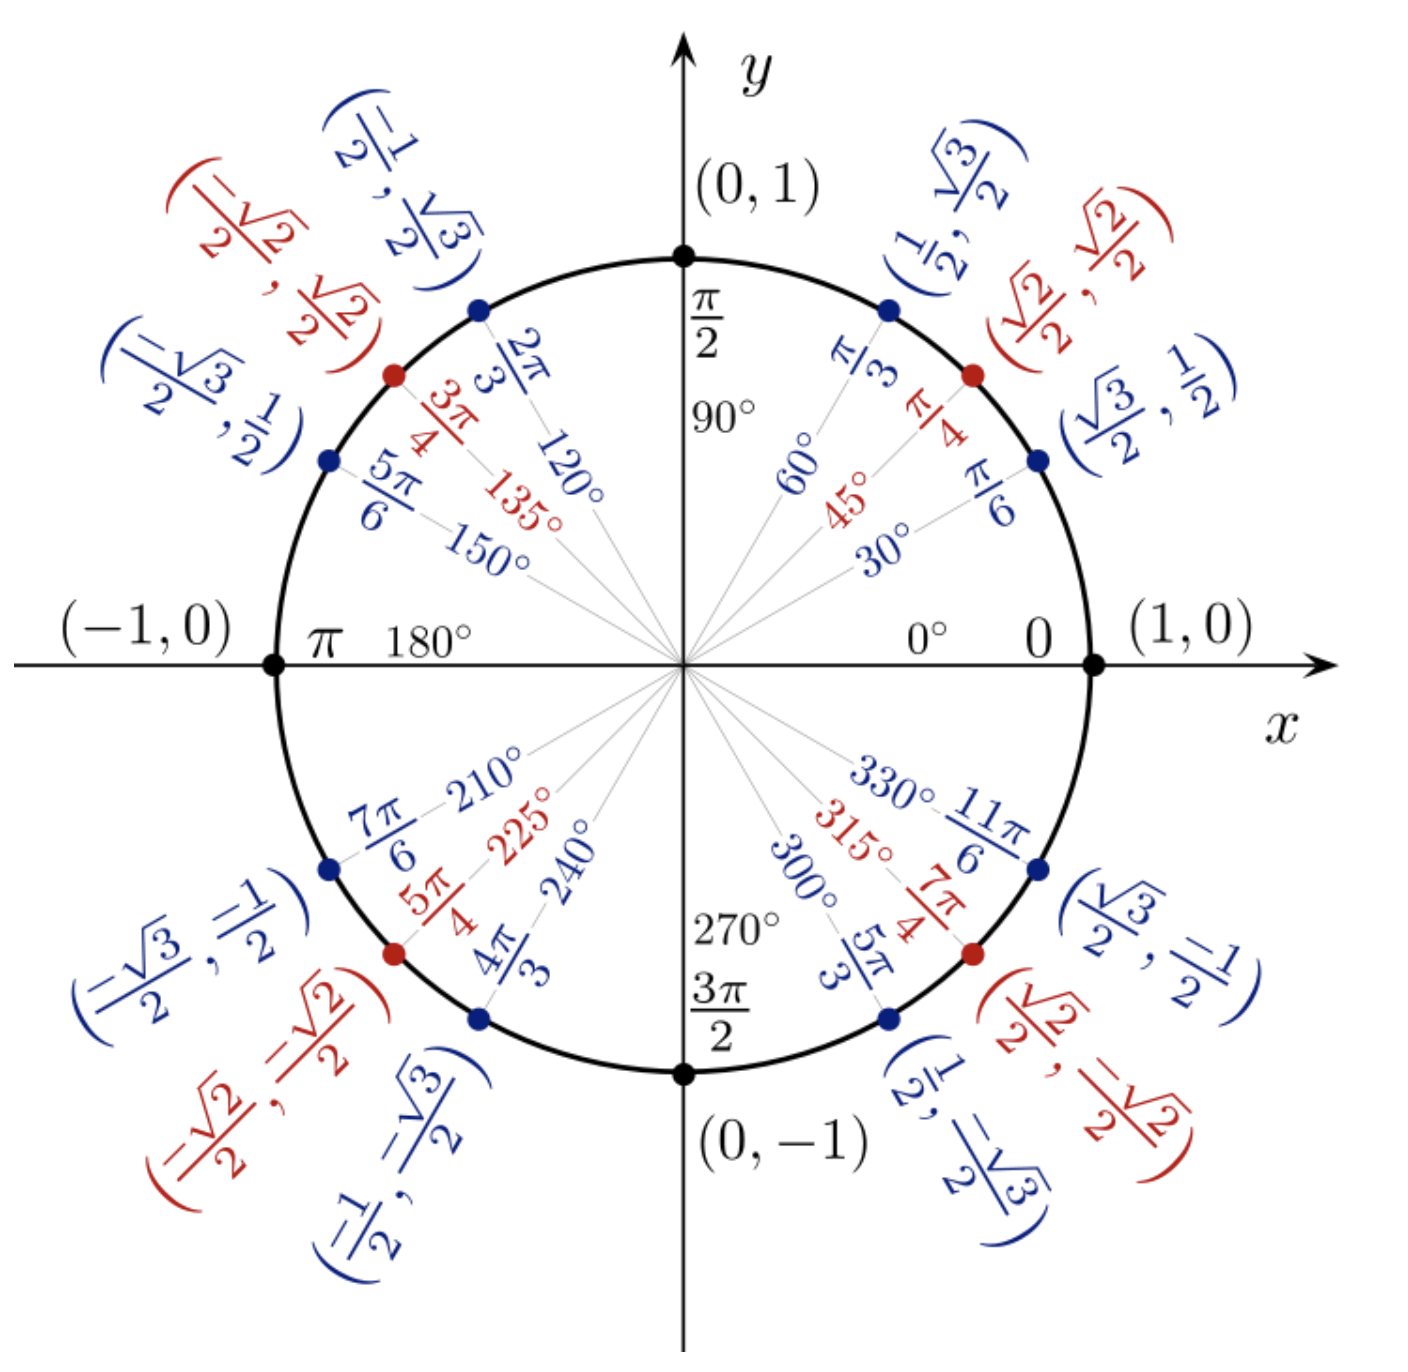
\includegraphics[width=0.5\linewidth]{Bilder/unit_circle.png}
    \caption{Unit Circle}
    \label{fig:unit_circle}
%Quelle : https://www.govst.edu/uploadedFiles/Academics/Colleges_and_Programs/CAS/Trigonometry_Short_Course_Tutorial_Lauren_Johnson.pdf%
\end{figure}

\subsection{Defining Sine, Cosine and Tangent}

The trigonometric functions Sine, Cosine and Tangent describe relationships between angles and side lengths in right-angled triangles. So let's start with some facts about right-angled triangles. The side opposite to the right-angle is called \textbf{hypothenuse}. If the length of the hypothenuse is called $c$ and the lengths of the two legs is given by $a$ and $b$, Pythagoras Theorem states that
\begin{equation}
    a^2+b^2=c^2.
\end{equation}

When considering an angle in a right triangle, the side of the triangle that touches the angle is called the \textbf{adjacent side}. The remaining third side is called \textbf{opposite side}. By the congruence theorem SSS, the length of hypothenuse, opposite and adjacent side define a unique right triangle. A triangle with labeled sides is shown in Fig. \ref{fig:right_angle_triangle}.

%Bild mit Hypothenuse, Gegen- und Ankathete, Bilder ähnlicherb Dreiecke%

\begin{figure}
    \centering
    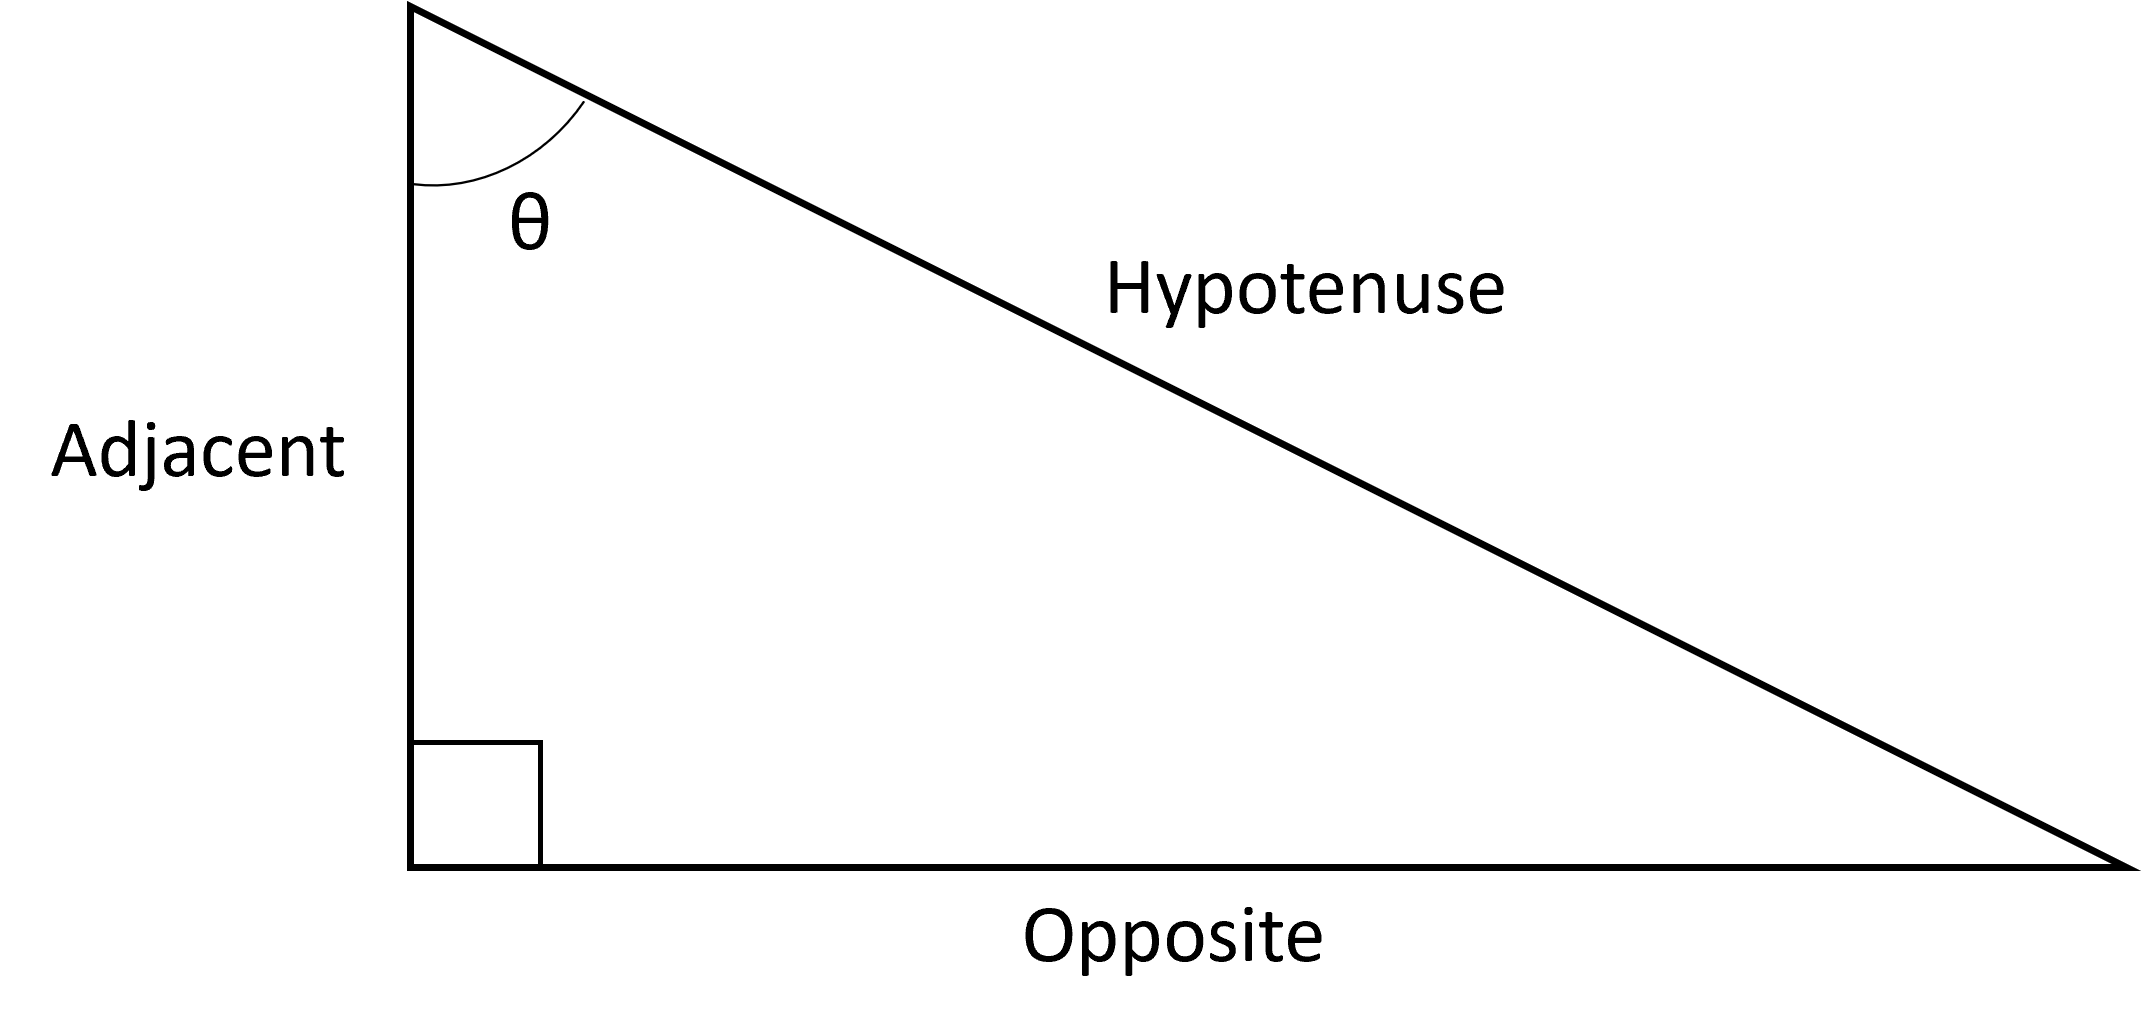
\includegraphics[width=0.5\linewidth]{Bilder/right_angled_triangle_labeled.png}
    \caption{A right angled triangle with labeled sides.}
    \label{fig:right_angle_triangle}
%Quelle : https://achievable-public-assets.s3.amazonaws.com/products/act/math/properties-trigonometric-functions/basic-trigonometry-triangle-hypotenuse-adjacent-side-opposite-side-theta-flipped.png
\end{figure}

We now consider similar right-angled triangles. Similar triangles have equal angles but different side lengths, so they are basically re-scaled copies of each other. 
We now observe that the ratio of the side lengths is the same for similar triangles. So for a certain angle $\alpha $, the following fundamental ratios don't depend on the size of a specific right-angled triangle. We define:
\begin{itemize}
    \item $\sin(\alpha) = \frac{\text{opposite}}{\text{hypotenuse}}$
    \item $\cos(\alpha) = \frac{\text{adjacent}}{\text{hypotenuse}}$
    \item $\tan(\alpha) = \frac{\text{opposite}}{\text{adjacent}}$
\end{itemize}
You can now also think of these equations as functions, where $\alpha$ is the variable. This means that, for a given angle, you are asking for the ratios of the side lengths of the corresponding right triangle. 
Trigonometric functions can be used to calculate missing side lengths and determine unknown angles.

To determine the values of $\sin(\alpha)$ and $\cos(\alpha)$ the unit circle can also be used: As you already know, the  unit circle is a circle with radius $1$ centered at the origin. An angle $\alpha$ is measured from the positive x-axis and corresponds to a certain point on the unit circle. To find the corresponding point on the circle, imagine rotating a radius of length 1 by the angle $\theta$. The endpoint of this radius lies on the circle and has coordinates $(x,y)$.

This construction forms a right triangle:
\begin{itemize}
    \item the hypotenuse is the radius $r=1$
    \item the horizontal side has length $x$
    \item the vertical side has length $y$
\end{itemize}

Using the definitions of trigonometric functions in a right triangle, one obtains:
\begin{equation}
    \cos(\alpha) = \frac{\text{adjacent}}{\text{hypotenuse}} = x
\end{equation}
\begin{equation}
    \sin(\alpha) = \frac{\text{opposite}}{\text{hypotenuse}} = y
\end{equation}

Thus, the point on the unit circle corresponding to the angle $\alpha$ is described by the coordinates: $(\sin(\alpha), \cos(\alpha))$. 
So for $\alpha = 45^\circ$, the triangle is isosceles, so both legs are equal. Considering the unit circle, one can easily determine $\sin(\alpha)$ and $\cos(\alpha)$:
\begin{equation}
    \cos(45^\circ) = \sin(45^\circ) = \frac{\sqrt{2}}{2}
\end{equation}

\textit{Question: What is $\sin(30^\circ)$? What about $\sin(5\pi/6)$? Use Fig. \ref{fig:unit_circle} to find the ratios. What about $\cos(120^\circ)$ and $\cos(4\pi/4)$? Do you notice something?}

\paragraph{Periodicity:}
The periodicity of sine and cosine function follows directly from the geometry of the unit circle. After a full rotation of $360^\circ$ (or $2\pi$ radians), the same  triangle is  created , and thus the point on the circle is identical. So, sine and cosine are periodic functions with a period of  $360^\circ$ (or $2\pi$ radians). 
In a more formal way, this is written as follows :
\begin{equation}
    \sin(\alpha + 2\pi) = \sin(\alpha), \quad \cos(\alpha + 2\pi) = \cos(\alpha)
\end{equation}

Another important identity is:
\begin{equation}
    \sin^2(x) + \cos^2(x) = 1
\end{equation}
This follows from the unit circle as well. The right triangles that are considered show the side lengths of sine and cosine while the length of the hypothenuse is 1. Thus, the identity is derived using this characteristics and Pythagoras Theorem.  




\subsection{Graphs of Trigonometric Functions}

Trigonometric functions can also be represented graphically.
As we saw in the last section, sine and cosine function are periodic with a period of $2\pi$. 
\paragraph{Sine function}
%Bild einer Sinus-Fkt. einfügen%
When plotting the sine function we get to know more properties of it: 

\begin{itemize}
    \item \textbf{Domain \footnote{all possible input values (what you can plug into the function)}}: $(-\infty, \infty)$  
    This means you can insert any real number into the function.

    \item \textbf{Range \footnote{all possible output values (what comes out of the function)}}: $[-1,1]$  
    The output values of the sine function are always between $-1$ and $1$.

    \item \textbf{x-intercepts \footnote{points where the graph touches or crosses the x-axis}}: $x = n\pi$, where $n \in \mathbb{Z}$  
    These are the points where the graph crosses the x-axis (i.e., where $\sin(x)=0$).
    \item \textbf{Periodicity}:  
    The sine function repeats itself every $2\pi$:
    \begin{equation}
        \sin(x + 2\pi) = \sin(x)
    \end{equation}
    \item \textbf{Odd function}:  
    The sine function is symmetric with respect to the origin. This means:
    \begin{equation}
        \sin(-x) = -\sin(x)
    \end{equation}

\end{itemize}



\paragraph{Cosine Function}
%P=lot von Cosinus einfügen %
When plotting the cosine function one observes similar properties:

\begin{itemize}
    \item \textbf{Domain}: $(-\infty, \infty)$  
    Any real number can be used as input.

    \item \textbf{Range}: $[-1,1]$  
    The values always stay between $-1$ and $1$.

    \item \textbf{Periodicity}:  
    The cosine function also repeats every $2\pi$:
    \begin{equation}
        \cos(x + 2\pi) = \cos(x)
    \end{equation}
    \item \textbf{Even function}:  
    The cosine function is symmetric with respect to the y-axis. This means:
    \begin{equation}
        \cos(-x) = \cos(x)
    \end{equation}

\end{itemize}

\paragraph{Explanation of Even and Odd Functions:}
\begin{itemize}
    \item \textbf{Even function}: The graph looks the same on the left and right side (mirror symmetry at the y-axis)
    \item \textbf{Odd function}: The graph looks the same after rotating it by $180^\circ$ around the origin
\end{itemize}
Both sine and cosine functions are periodic and oscillate between $-1$ and $1$. This makes them especially useful for describing waves and oscillations in physics.

\subsection{Transformations of Sine and Cosine Functions}

Sine and cosine functions can be modified using parameters. The general form of such a function is:

\begin{equation}
    f(x) = a \cdot \sin(bx + c) + d \quad \text{or} \quad f(x) = a \cdot \cos(bx + c) + d
\end{equation}

Each parameter changes the graph in a specific way:

\begin{itemize}
    \item \textbf{Amplitude ($a$):}  
    The amplitude describes how ``tall'' the wave is. It tells you the maximum distance from the middle line (equilibrium).
    \begin{itemize}
        \item $|a| > 1$: the graph is stretched (bigger peaks)
        \item $0 < |a| < 1$: the graph is compressed (smaller peaks)
        \item $a < 0$: the graph is reflected across the x-axis
    \end{itemize}

    \item \textbf{Period ($b$):}  
    The parameter $b$ changes how long one full wave lasts.
    The period $T$ is given by:
    \begin{equation}
        T = \frac{2\pi}{b}
    \end{equation}
    \begin{itemize}
        \item $b > 1$: the wave is compressed (repeats faster)
        \item $0 < b < 1$: the wave is stretched (repeats slower)
    \end{itemize}

    \item \textbf{Phase shift ($c$):}  
    The phase shift moves the graph left or right.
    \begin{equation}
        \text{shift} = -\frac{c}{b}
    \end{equation}
    \begin{itemize}
        \item shift to the right if $c < 0$
        \item shift to the left if $c > 0$
    \end{itemize}

    \item \textbf{Vertical shift ($d$):}  
    The parameter $d$ moves the whole graph up or down.
    \begin{itemize}
        \item $d > 0$: graph shifts upward
        \item $d < 0$: graph shifts downward
    \end{itemize}
\end{itemize}

\paragraph{How to think about it :}
\begin{itemize}
    \item The \textbf{amplitude} tells you how strong the oscillation is.
    \item The \textbf{period} tells you how long it takes until the wave repeats.
    \item The \textbf{phase shift} tells you where the wave starts.
    \item The \textbf{vertical shift} moves the whole wave up or down.
\end{itemize}

\subsection{Relationship Between Sine and Cosine}

The sine and cosine functions are closely related and can be transformed into each other by a simple horizontal shift. In fact, they describe the same type of oscillation, but start at different points.

The relationship is given by:
\begin{equation}
    \cos(x) = \sin\left(x + \frac{\pi}{2}\right)
\end{equation}
\begin{equation}
    \sin(x) = \cos\left(x - \frac{\pi}{2}\right)
\end{equation}

This means that the cosine function is just the sine function shifted to the left by $\frac{\pi}{2}$ (a quarter of a full period), and vice versa.

\paragraph{How to think about it :}
\begin{itemize}
    \item Both functions describe the same wave shape.
    \item The only difference is where the wave starts.
    \item A shift of $\frac{\pi}{2}$ moves the starting point from a maximum (cosine) to a zero crossing (sine).
\end{itemize}

\paragraph{Summary:}
By changing the parameters $a$, $b$, $c$, and $d$, we can model many different types of waves and oscillations. This is especially important in physics, for example when describing sound waves or vibrations.